\documentclass[tikz,border=10pt]{standalone}
\usepackage{tikz}
\usepackage{amsmath}
\usetikzlibrary{shapes.geometric, arrows.meta, positioning, calc}

\begin{document}
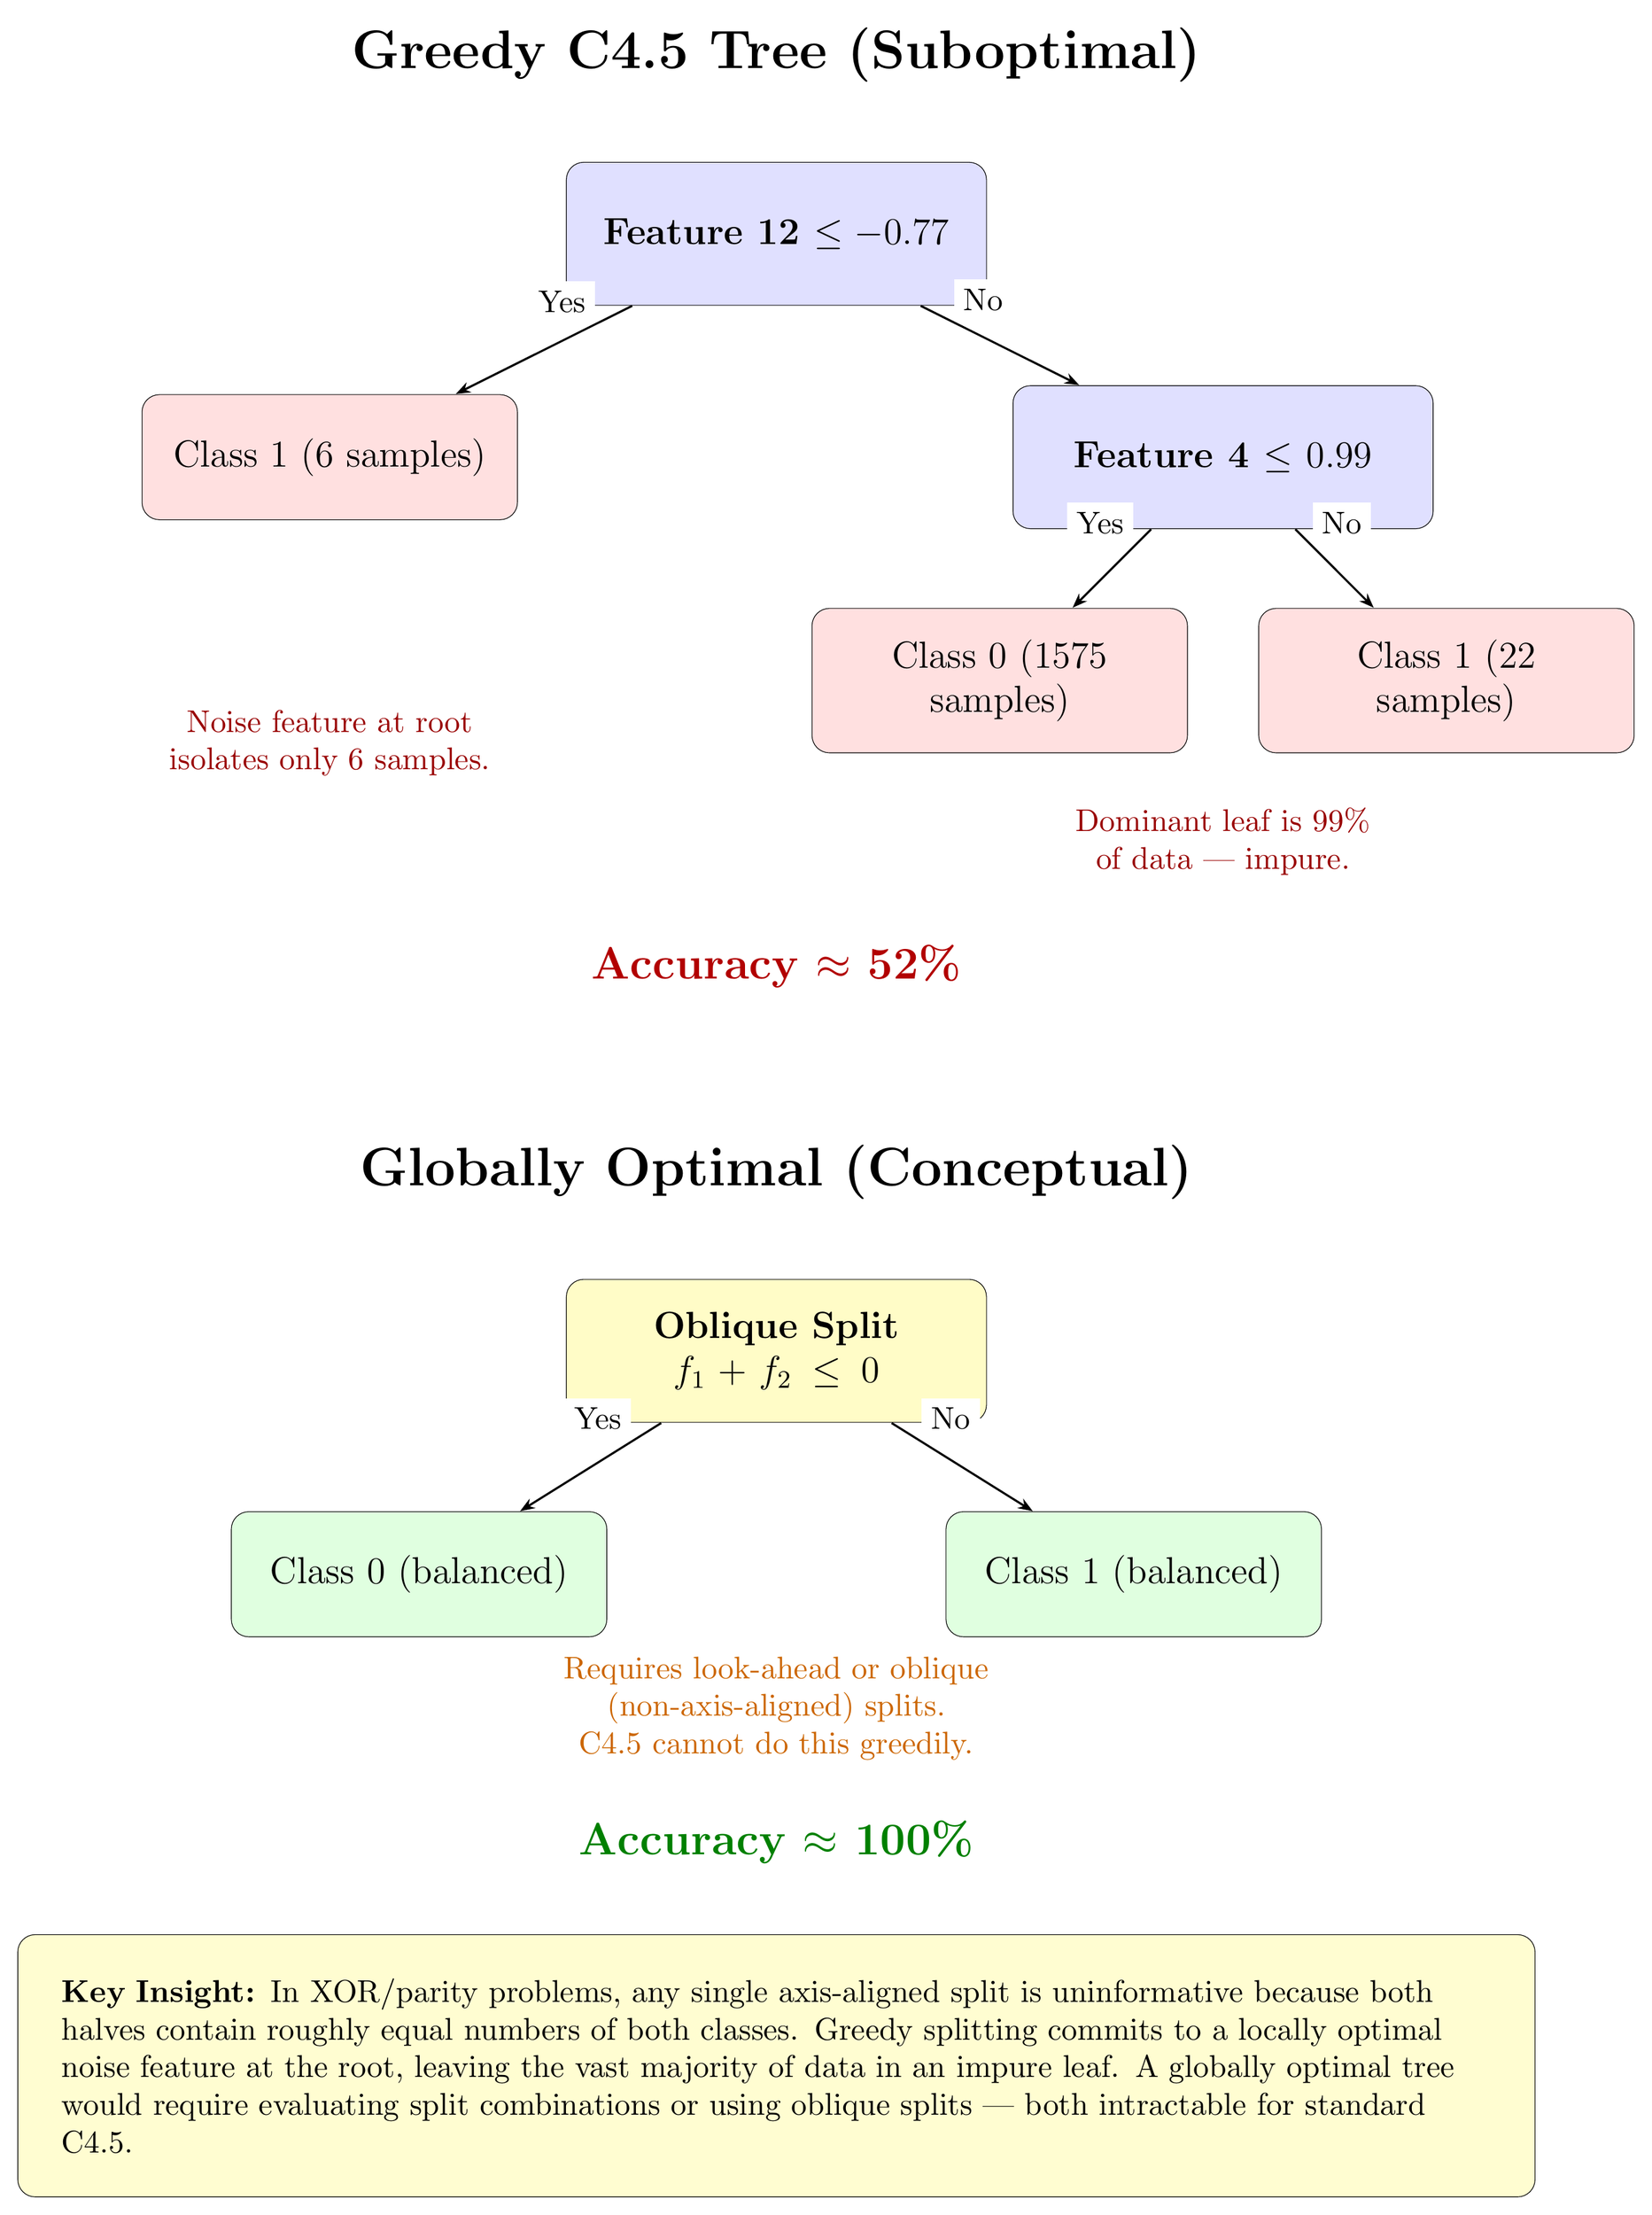
\begin{tikzpicture}[
    scale=1.8,
    transform shape,
    node distance=2.2cm and 4cm,
    every node/.style={font=\large},
    decision/.style={
        rectangle,
        rounded corners=10pt,
        draw=black,
        fill=blue!12,
        text width=4cm,
        minimum height=1.6cm,
        align=center,
        inner sep=10pt,
        font=\large\bfseries
    },
    leaf/.style={
        rectangle,
        rounded corners=10pt,
        draw=black,
        fill=green!12,
        text width=3.5cm,
        minimum height=1.4cm,
        align=center,
        inner sep=10pt,
        font=\large
    },
    badleaf/.style={
        rectangle,
        rounded corners=10pt,
        draw=black,
        fill=red!12,
        text width=3.5cm,
        minimum height=1.4cm,
        align=center,
        inner sep=10pt,
        font=\large
    },
    oblique/.style={
        rectangle,
        rounded corners=10pt,
        draw=black,
        fill=yellow!22,
        text width=4cm,
        minimum height=1.6cm,
        align=center,
        inner sep=10pt,
        font=\large\bfseries
    },
    arrow/.style={
        ->,
        >=Stealth,
        very thick,
        black
    },
    edgelabel/.style={
        font=\normalsize,
        fill=white,
        inner sep=3pt
    }
]

% ============================================
% TOP: Greedy C4.5 Tree (Suboptimal)
% ============================================
\node[font=\LARGE\bfseries] at (0,8) {Greedy C4.5 Tree (Suboptimal)};

\node[decision] (root) at (0,6) {Feature 12 $\leq -0.77$};

\node[badleaf] (l1) at (-5,3.5) {Class 1 (6 samples)};
\node[decision] (r1) at (5,3.5) {Feature 4 $\leq 0.99$};

\node[badleaf] (rl2) at (2.5,1) {Class 0 (1575 samples)};
\node[badleaf] (rr2) at (7.5,1) {Class 1 (22 samples)};

\draw[arrow] (root) -- node[edgelabel, above left, pos=0.2] {Yes} (l1);
\draw[arrow] (root) -- node[edgelabel, above right, pos=0.2] {No} (r1);
\draw[arrow] (r1) -- node[edgelabel, above left, pos=0.2] {Yes} (rl2);
\draw[arrow] (r1) -- node[edgelabel, above right, pos=0.2] {No} (rr2);

% Annotations
\node[font=\normalsize, text width=4.5cm, align=center, color=red!60!black] at (-5,0.3) {
    Noise feature at root isolates only 6 samples.
};

\node[font=\normalsize, text width=4.5cm, align=center, color=red!60!black] at (5,-0.8) {
    Dominant leaf is 99\% of data --- impure.
};

\node[font=\Large\bfseries, color=red!70!black] at (0,-2.2) {Accuracy $\approx$ 52\%};

% ============================================
% BOTTOM: Globally Optimal Concept
% ============================================
\node[font=\LARGE\bfseries] at (0,-4.5) {Globally Optimal (Conceptual)};

\node[oblique] (oroot) at (0,-6.5) {Oblique Split $f_1 + f_2 \leq 0$};

\node[leaf] (ol1) at (-4,-9) {Class 0 (balanced)};
\node[leaf] (ol2) at (4,-9) {Class 1 (balanced)};

\draw[arrow] (oroot) -- node[edgelabel, above left, pos=0.2] {Yes} (ol1);
\draw[arrow] (oroot) -- node[edgelabel, above right, pos=0.2] {No} (ol2);

\node[font=\normalsize, text width=6cm, align=center, color=orange!80!black] at (0,-10.5) {
    Requires look-ahead or oblique (non-axis-aligned) splits. C4.5 cannot do this greedily.
};

\node[font=\Large\bfseries, color=green!50!black] at (0,-12) {Accuracy $\approx$ 100\%};

% ============================================
% Bottom insight box
% ============================================
\node[draw=black, fill=yellow!18, text width=16cm, align=left, inner sep=14pt, rounded corners=10pt, font=\normalsize] at (0,-14.5) {
    \textbf{Key Insight:} In XOR/parity problems, any single axis-aligned split is uninformative because both halves contain roughly equal numbers of both classes. Greedy splitting commits to a locally optimal noise feature at the root, leaving the vast majority of data in an impure leaf. A globally optimal tree would require evaluating split combinations or using oblique splits --- both intractable for standard C4.5.
};

\end{tikzpicture}
\end{document}
